\documentclass[a4paper]{article}
\usepackage[UTF8]{ctex}
\usepackage{geometry}
\usepackage{graphicx}
\usepackage{url}
\usepackage{multirow}
\usepackage{array}
\usepackage{booktabs}
\usepackage{url}
\usepackage{enumitem}
\usepackage{graphicx}
\usepackage{float}
\usepackage{amssymb}
\usepackage{amsmath}
\usepackage{subfig}
\usepackage{longtable}
\usepackage{pifont}
\usepackage{color}

\allowdisplaybreaks

\geometry{a4paper, scale=0.78}

% \begin{figure}[H]
%     \centering
%     \includegraphics[width=.55\textwidth]{E.png}
%     \caption{矩阵与列向量的乘法}
%     \label{fig:my_label_1}
% \end{figure}

% \left\{
% \begin{array}{ll}
%       x+2x+z=2 & \\
%       3x+8y+z=12 & \\
%       4y+z=2
% \end{array}
% \right.

% \begin{enumerate}[itemindent = 1em, itemsep = 0.4pt, parsep=0.5pt, topsep = 0.5pt]

% \end{enumerate}

%\stackrel{a}{\longrightarrow}

\title{Probability Graph 09 Max Product Algorithm}
\author{Chen Gong}
\date{10 December 2019}

\begin{document}
\maketitle
我们在这里再总结一下概率图模型有什么用。对于一个图,Graph = $\{ X,E \}$,其中$X$代表的是普通变量,$E$代表的是Evidence,也就是观测变量。

1. 首先要解决的是边缘变量的问题,也就是已知:$E=\{ e_1,e_2,\cdots,e_k \}$,如何求$p(E)$的问题,其中$E$为一个变量或者为一个子集。实际上就是一个likelihood的问题。

2. 条件概率,也就是一个求后验概率的问题,目标概率为$X=(Y,Z)$。而$p(Y|E) = \sum_z p(X|E)$。

3. 最大后验估计(MAP),也被我们称为Decoding的问题。也就是我们希望找到一个隐序列,使得:$\hat{x} = argmax_x p(X|E)$,$\hat{y} = argmax_y p(Y|E)$。

这里的Max-Product算法和隐马尔可夫模型(HMM)中的Viterbi算法非常的类似。其实,从算法上讲它就是Belief Propagation算法的一种改进,从模型上讲是Viterbi算法的推广。在这里我们求的不是概率值了,而是一个最优的概率序列$(\hat{a},\hat{b},\hat{c},\hat{d}) = argmax_{a,b,c,d}p(x_a,x_b,x_c,x_d|E)$。

\section{Max Product Algorithm}
下面展示一个树的拓扑结构图。
\begin{figure}[H]
    \centering
    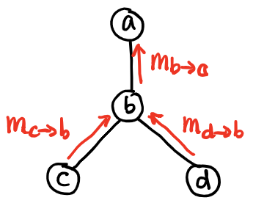
\includegraphics[width=.35\textwidth]{微信图片_20191210100004.png}
    \caption{概率树模型的拓扑结构图}
    \label{fig:my_label_1}
\end{figure}

在这个树中,我们将$m_{b \longrightarrow a}$看成是能使$p(x_b,x_c,x_d|E)$联合概率达到最大的值。每一个节点代表的是到这个节点为止的路径联合概率达到最大的值。我们表达为:
\begin{equation}
    m_{j\longrightarrow i} = \max_{x_j} \varphi_i\varphi_{ij}\prod_{k\in \{NB(j)-i\}}m_{k \longrightarrow j}
\end{equation}

那么,在图一所示的概率图模型中,$m_{c\longrightarrow b}$可以表示为:
\begin{equation}
    m_{c\longrightarrow b}=\max_{x_c} \varphi_c\cdot \varphi_{bc}
\end{equation}

其中,$\varphi_c\cdot \varphi_{bc}$可以表示为和$c$相关的函数。
\begin{equation}
    m_{d\longrightarrow b}=\max_{x_d} \varphi_c\cdot \varphi_{cd}
\end{equation}

其中,$\varphi_d\cdot \varphi_{cd}$可以表示为和$d$相关的函数。
\begin{equation}
    m_{b\longrightarrow a} = \max_{x_b} \varphi_b \cdot \varphi_{ab}\cdot m_{c\longrightarrow b}\cdot m_{d\longrightarrow b}
\end{equation}

最终,我们将得到的是:
\begin{equation}
    \max p(a,b,c,d) = \max_{x_a} \varphi_a m_{b\longrightarrow a}
\end{equation}

而$\varphi_a m_{b\longrightarrow a}$就可以看成是一个关于$a$的函数。这里我们再提一下Belief Propagation,这里的Max-Product实际上就是Belief Propagation的一个变形。

\section{Belief Propagation}
实际上这个算法的提出时因为,多次求边缘概率密度会发现中间有很多的步骤是重复的。我们用$m_{i\longrightarrow j}$记录每一个边缘概率,最后进行组合就行。所以,
\begin{equation}
    m_{j\longrightarrow i}(x_i) = \sum_{x_j} \varphi_{i,j}(x_i,x_j)\varphi_j(x_j) \prod_{\{k \in NB(j)\}\longrightarrow i } m_{k\longrightarrow j}(x_j)
\end{equation}

而:
\begin{equation}
    p(x_i) = \varphi(x_i) \prod_{k \in NB(x_i)} m_{k\longrightarrow i}(x_i)
\end{equation}

\section{Compare}
其实,我们一比较就可以很简单的看出,Max-product和Belief Propagation只有一个地方不一样。那就是前者是求最大,后者是求和。也就是Max-product到Sum-product。在求得了$\max p(a,b,c,d) = \max_{x_a} \varphi_a m_{b\longrightarrow a}$之后,我们利用回溯法我们比较就可以比较简单的得到$x_a^\ast,x_b^\ast,x_c^\ast,x_d^\ast$了。在这个算法中,我们就不需要事先计算$m_{i\longrightarrow j}$了,直接在迭代中进行计算就可以了,也不会存在什么重复计算的问题。

\end{document}
